\chapter{Implementierung}\label{chap:Implementierung}
\thispagestyle{standard}
\pagestyle{standard}
\lfoot{\small Refik Kerimi}

\section{Umsetzung der Anforderungen}\label{sub:Umsetzung der Anforderungen}
In diesem Kapitel wird die Umsetzung der Applikation beschrieben. Die Anforderungen aus Kapitel \ref{sub:Anforderungsanalyse}
Zur Erstellung des User Interfaces wird ReactJS\footnote{https://reactjs.org/docs/getting-started.html} und als CSS Framework Semantic-UI\footnote{https://react.semantic-ui.com/introduction} verwendet, Sematic-UI soll sicherstellen das die Applikation responives verhalten aufweist und für alle Bildschirmgrößen geeignet ist. Um die Daten zu versenden, aufzurufen und zu speichern wurde das JSON Key/Value Format, die Fetch API und der Browser Cache verwendet.
Als Browser wurde der Google Chrome Version 67 verwendet.
Die nicht fertigen Funktionen wurden mit Mockups dargestellt um einen Eindruck zu vermitteln wie das ganze in Zukunft aussehen soll.

\section{Ausgewählte Programmiersprache und IDE}
Als Programmiersprache wurde \acl{JS} (\acs{JS}) ausgewählt. 
Als Entwicklungsumgebung wurde Webstorm (Version 2018.2) von Jetbrains verwendet. 
Weitere verwendete Tools und Frameworks wurden im Kapitel \ref{sub:Umsetzung der Anforderungen} beschrieben.
\newpage
\section{Ordnerstruktur}
Die zwei wichtigsten Dateien befinden sich wie der Abbildung \ref{fig:OrderStrucktur} zu sehen im App Verzeichnis.
Weiters wichtig ist das app.js File dieses ist unter \textit{/app/src/js/app.js} zu finden.

\begin{figure}[h]
	\centering
	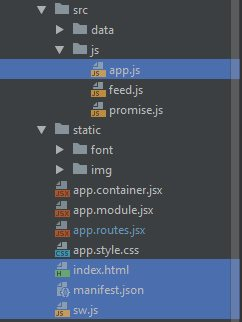
\includegraphics[width=10cm]{BilderAllgemein/Implementierung/OrdnerStrucktur.jpg}\medskip
	\caption{Ordner Strucktur}
	\label{fig:OrdnerStrucktur}
\end{figure} 


\section{Manifest}
Das Manifest wird im Root Folder eingafügt und ist mit der Endung JSON deklariert. Der genau Pfad ist \textit{/app/manifest.json}. Wie im Kapitel \ref{sub:Manifest} schon beschrieben definiert das manifest File das Aussehen des Startbildschirm Icons, den Einstiegspunkt der App und weiter Attribute, die im Listening \ref{lst:Manifest.json} zu sehen sind:
\newpage
\begin{lstlisting}[language=json, firstnumber=1, caption={Manifest in das Projekt implementieren} {\cite{Manifest}},label=lst:Manifest.json, xleftmargin=50pt]
{
  {
  "name":"PWA Smart Home",
  "short_name":"PWA_SHL_RMJ",
  "start_url":"./",
  "scope":".",
  "display":"standalone",
  "background_color":"#003399",
  "theme_color":"#3F51C5",
  "description":"Keep running with PWA",
  "dir":"ltr",
  "lang":"de-DE",
  "orientation":"portrait-primary",
  "icons":[
    {
      "src":"./static/img/light48.png",
      "type":"image/png",
      "sizes":"48x48"
    },
    {
      "src":"./static/img/light512.png",
      "type":"image/png",
      "sizes":"512x512"
    }
  ]
}
}
\end{lstlisting}

\section{Add to Homescreen}
Wie in Kapitel \ref{sub:AddtoHomescreen} muss damit der Add to Homescreen Banner erscheint die Bedingungen erfüllen.
Nach erfüllung dieser Forderungen wird der beforeinstallprompt Event wie in Listening \ref{lst:AddtoHomescreen} aufgerufen und in die deferredPrompt variable gespeichert.

\begin{lstlisting}[language=JavaScript, firstnumber=1, caption={Add to Homescreen Funktion} ,label=lst:AddtoHomescreen, xleftmargin=50pt]
var deferredPrompt;

window.addEventListener('beforeinstallprompt', event => {
    event.preventDefault();
    deferredPrompt = event;
    return false;
});
%\end{lstlisting}

Diese Standardfunktion wird in die app.js Datei implementiert. 

\section{Service Worker und Cache API}
Das Herzstück der Applikation ist der im Kapitel Basistechnologien beschriebene Service Worker. Als erstes muss Validiert werden ob der Service Worker vom Browser unterstützt wird und danach wird dieser registriert, installiert und aktiviert.
In den folgenden Listings \ref{lst:Registrierung}, \ref{lst:Installation} und \ref{lst:Aktivierung}, sind die Funktionen angegeben die für den \acs{SW} von Bedeutung sind aufgeführt und die wichtigsten Teile beschrieben.

Verzeichnis: \textit{/app/src/js/app.js}

\begin{lstlisting}[language=JavaScript, firstnumber=1, caption={Registrierung} ,label=lst:Registrierung, xleftmargin=50pt]
//Registrierung und Validierung vom Service Worker
if ('serviceWorker' in navigator) {
    console.log('Service Worker and Notification is supported')
    navigator.serviceWorker.register('/sw.js')
        .then(reg => {
            console.log('Service worker registered!', reg);

        })
        .catch(err => console.log(err));
}
\end{lstlisting}
Die Registriermethode \textit{register()} bekommt als Parameter die Service Worker Datei mitgegeben.

Verzeichnis: \textit{/app/sw.js}

\begin{lstlisting}[language=JavaScript, firstnumber=1, caption={Installation} ,label=lst:Installation, xleftmargin=50pt]
self.addEventListener('install', event => {
    console.log('[Service Worker] Installing Service Worker ....', event);
    event.waitUntil(
        caches.open(cacheName)
            .then(cache => {
                console.log('[Service Worker] Precaching App Frame');
                cache.addAll(filesToCache);
            })
    )
});
}
\end{lstlisting}

Nach dem erneuten Laden der Anwenung wird der Installation Eventlistener aufgerufen. Dieser Installiert den Service Worker und cached die Angegebenen Dateien um die App offline verwenden zu können. 

Verzeichnis: \textit{/app/sw.js}

\begin{lstlisting}[language=JavaScript, firstnumber=1, caption={Installation} ,label=lst:Installation, xleftmargin=50pt]
self.addEventListener('install', event => {
    console.log('[Service Worker] Installing Service Worker ....', event);
    event.waitUntil(
        caches.open(cacheName)
            .then(cache => {
                console.log('[Service Worker] Precaching App Frame');
                cache.addAll(filesToCache);
            })
    )
});
}
\end{lstlisting}

Durch die Funktion \textit{waitUntil()} wird mit der Installation gewartet bis die Datei die dieser Funktion als Parameter mitgegeben wurden gecachte wurden. Durch die Cachemethode \textit{cache.All()} werden alle angegeben Dateien aufgerufen und man muss nicht alle Dateien einzeln eingeben.
Nach der Installation wird der Service Worker aktiviert und kann dan vom Browser verwendet werden.

Verzeichnis: \textit{/app/sw.js}

\begin{lstlisting}[language=JavaScript, firstnumber=1, caption={Aktivierung} ,label=lst:Aktivierung, xleftmargin=50pt]
self.addEventListener('activate', event => {
    console.log('[Service Worker] Activating Service Worker ....', event);
    return self.clients.claim();
})
\end{lstlisting}

Durch die \textit{self.clients.claim()} Methode in Zeile 3 wird sichergestellt das der Service Worker nur installiert wird wenn alle Bedingungen erfüllt worden sind.

Weiters wichtig ist die fetch-Methode. Diese Methode ruft Daten im Key:Value Format entweder vom Cache oder falls die Daten nicht im Cache vorhanden sind vom Webserver.

Verzeichnis: \textit{/app/sw.js}

\begin{lstlisting}[language=JavaScript, firstnumber=1, caption={Aktivierung} ,label=lst:Aktivierung, xleftmargin=50pt]
self.addEventListener('fetch', event => {
    event.respondWith(
        caches.match(event.request)
            .then(response => {
                if (response) {
                    return response;
                }else{
                    return fetch(event.request);
                }
            })
    );
});
\end{lstlisting}

Der Callback-Funktion \textit{respondWith()} werden die Daten aufgerufen die match-Methode überprüft ob die Daten sich im Cache befinden.

		
Notizen Video
	Asynchronus Code Abschitt 6 Lektion 62 4:34 
	 

\section{Offline Modus}
Eine der Aufgaben des Caches vom Service Worker ist der Offlinemodus oder das Arbeiten bei schlechter Internetverbindung. Der Cache  beinhaltet im Grunde das Index.html File CSS und Bilder oder Icons. Bei der Entwicklung der Anwendung wurden statische Dateien wie im Listening \ref{lst:Cache} verwendet.


\begin{lstlisting}[language=JavaScript, firstnumber=1, caption={Cache} ,label=lst:Cache, xleftmargin=50pt]
let filesToCache = [
    '/',
    '/index.html',
    '/src/js/app.js',
    '/static/img/light48.png',
    '/static/img/dashboard-mockup.jpg',
    '/static/img/bulp.jpeg',
    '/static/img/garage.jpeg',
    '/static/img/Graph_Heizung.JPG',
    '/manifest.json'
];
\end{lstlisting}


\begin{figure}[h]
	\centering
	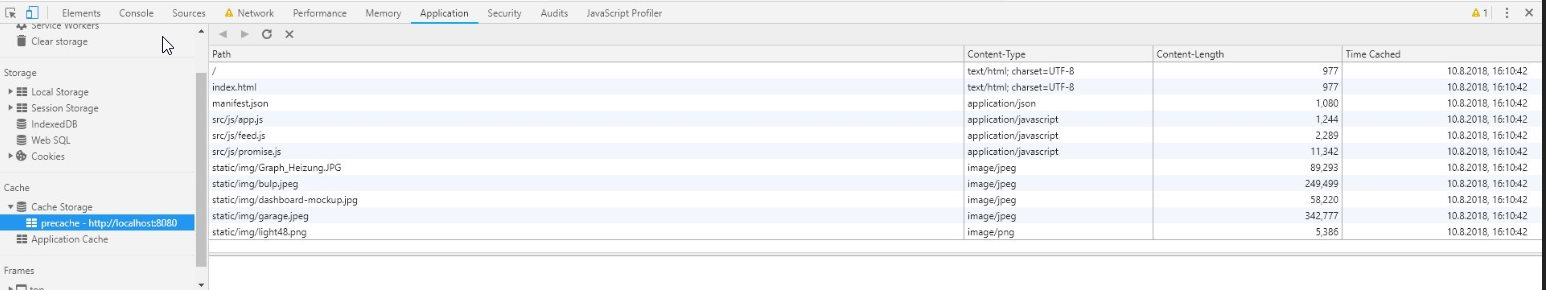
\includegraphics[width=16cm]{BilderAllgemein/Implementierung/Cache.jpg}\medskip
	\caption{Cache}
	\label{fig:Cache}
\end{figure}  

\begin{figure}[h]
	\centering
	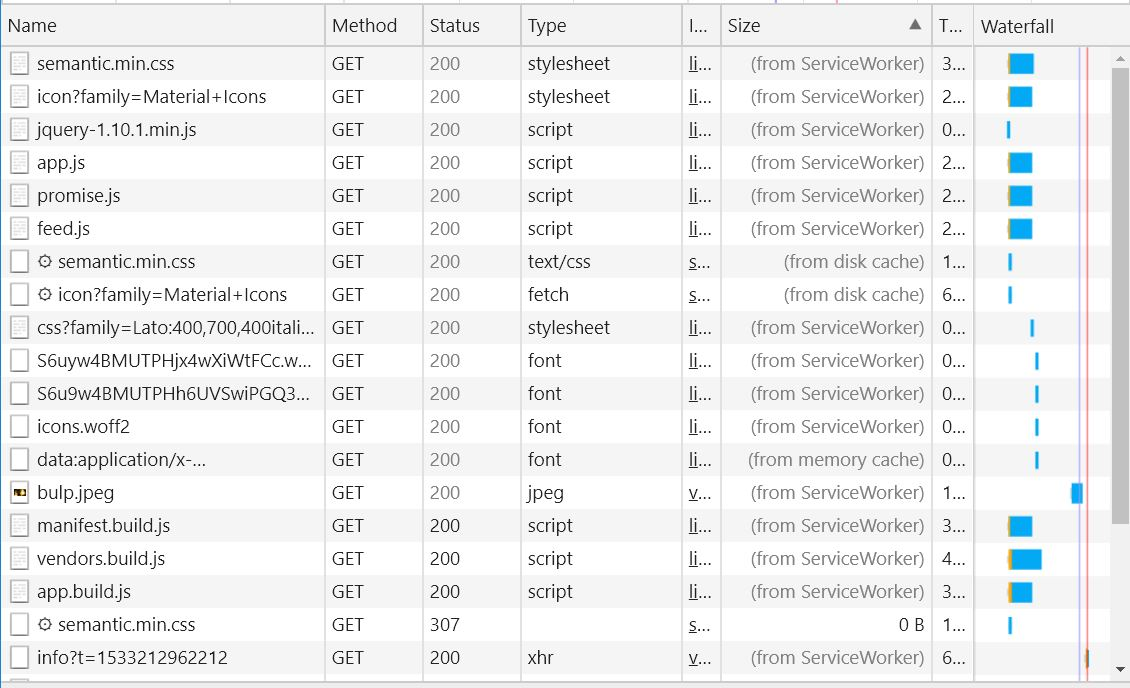
\includegraphics[width=8cm]{BilderAllgemein/Implementierung/aufruf_SW_Browser.jpg}\medskip
	\caption{Datenaufruf Service Worker}
	\label{fig:aufrufSWBrowser}
\end{figure}  

In der Abbildung \ref{fig:aufrufSWBrowser} und \ref{fig:Cache} kann man die gecachten Files vom Service Worker im Netzwerk und im Browsercache erkennen.

\section{Push Notifications}


\section{Geolocation API}











